%========================================================
% Experiment 2 — Two-Arm PMD and Spectral Correlations
%========================================================

%--------------------------------------------------------
% Objective and physical motivation
%--------------------------------------------------------

\subsection{Objective and Physical Motivation}

Experiment~1 isolated the elementary decoherence mechanism produced by PMD in a
single arm. The present experiment extends the analysis to the case in which both
photons propagate through frequency-dependent birefringent elements and investigates
the additional role of correlations in the two-photon spectrum.

The main objective is to determine whether the spectral correlation between the
frequency offsets of the two photons can modify the degradation of polarization
entanglement produced by two-arm PMD.

The reference polarization state is again

\begin{equation}
|\Psi^+\rangle
=
\frac{1}{\sqrt{2}}
\left(
|01\rangle + |10\rangle
\right).
\label{eq:exp2_input_bell_state}
\end{equation}

Both arms are assigned the same differential group delay,

\begin{equation}
\tau_A=\tau_B=\tau,
\label{eq:exp2_equal_dgd}
\end{equation}

while their birefringence axes are chosen to be opposite,

\begin{equation}
\hat{\mathbf n}_A=+\hat{\mathbf z},
\qquad
\hat{\mathbf n}_B=-\hat{\mathbf z}.
\label{eq:exp2_opposite_axes}
\end{equation}

The carrier-frequency differential phases are set to zero, so that the experiment
isolates the frequency-dependent contribution responsible for PMD.

%--------------------------------------------------------
% Spectral model and analytical prediction
%--------------------------------------------------------

\subsection{Spectral Model and Analytical Prediction}

The two photons are assigned equal marginal angular-frequency standard deviations

\begin{equation}
\sigma_A=\sigma_B=\sigma_\omega,
\end{equation}

while their joint spectrum is varied through the spectral correlation coefficient

\begin{equation}
r
=
\frac{
\operatorname{Cov}(\Omega_A,\Omega_B)
}{
\sigma_\omega^2
}.
\label{eq:exp2_spectral_correlation_coefficient}
\end{equation}

The Gaussian widths along the sum and difference frequency coordinates are therefore

\begin{align}
\sigma_{\mathrm{sum}}^2
&=
2\sigma_\omega^2(1+r),
\\
\sigma_{\mathrm{difference}}^2
&=
2\sigma_\omega^2(1-r).
\label{eq:exp2_sum_difference_widths}
\end{align}

Negative values of \(r\) correspond to frequency anticorrelation, \(r=0\) to an
uncorrelated joint spectrum, and positive values to positively correlated frequency
offsets.

For the configuration in Eq.~\eqref{eq:exp2_opposite_axes}, the frequency-dependent
relative phase accumulated between the two components of the Bell state is

\begin{equation}
\theta(\Omega_A,\Omega_B)
=
\tau(\Omega_A+\Omega_B).
\label{eq:exp2_relative_spectral_phase}
\end{equation}

Its variance is consequently

\begin{align}
\operatorname{Var}(\theta)
&=
\tau^2
\operatorname{Var}(\Omega_A+\Omega_B)
\nonumber
\\
&=
2\sigma_\omega^2\tau^2(1+r).
\label{eq:exp2_phase_variance}
\end{align}

For a zero-mean Gaussian spectrum, spectral averaging therefore gives the residual
polarization coherence

\begin{equation}
g(\tau,r)
=
\left\langle
e^{i\theta}
\right\rangle
=
\exp
\left[
-\sigma_\omega^2\tau^2(1+r)
\right].
\label{eq:exp2_coherence}
\end{equation}

Introducing the normalized PMD strength

\begin{equation}
\xi=\sigma_\omega\tau,
\label{eq:exp2_xi}
\end{equation}

the result becomes

\begin{equation}
\boxed{
g(\xi,r)
=
e^{-(1+r)\xi^2}
}.
\label{eq:exp2_coherence_normalized}
\end{equation}

After tracing over the unresolved spectral degrees of freedom, the polarization state
takes the form

\begin{equation}
\rho_{AB}(\xi,r)
=
\frac{1}{2}
\begin{pmatrix}
0 & 0 & 0 & 0
\\
0 & 1 & g & 0
\\
0 & g & 1 & 0
\\
0 & 0 & 0 & 0
\end{pmatrix}.
\label{eq:exp2_reduced_polarization_state}
\end{equation}

The principal analytical quantities follow directly:

\begin{align}
C
&=
g,
\\
F_{\Psi^+}
&=
\frac{1+g}{2},
\\
\gamma(\rho_{AB})
&=
\frac{1+g^2}{2},
\\
\gamma(\rho_A)
=
\gamma(\rho_B)
&=
\frac{1}{2},
\\
S_{\max}
&=
2\sqrt{1+g^2}.
\label{eq:exp2_analytical_metrics}
\end{align}

The correlation tensor is

\begin{equation}
T(\xi,r)
=
\begin{pmatrix}
g & 0 & 0
\\
0 & g & 0
\\
0 & 0 & -1
\end{pmatrix},
\label{eq:exp2_correlation_tensor}
\end{equation}

showing that PMD suppresses the transverse polarization coherence while the
longitudinal anticorrelation remains unchanged.

%--------------------------------------------------------
% Numerical configuration
%--------------------------------------------------------

\subsection{Numerical Configuration}

The numerical experiment evaluates the frequency-resolved two-photon state on a
uniform joint spectral grid and subsequently performs the discrete spectral trace.
The parameters used in the simulation are summarized in
Table~\ref{tab:exp2_numerical_configuration}.

\begin{table}[htbp]
    \centering
    \caption{Numerical configuration of Experiment~2.}
    \label{tab:exp2_numerical_configuration}

    \begin{tabular}{lc}
        \hline
        Parameter & Value
        \\
        \hline

        Marginal bandwidth \(\sigma_\omega\)
        & \(1.0\times10^{11}\,\mathrm{rad/s}\)
        \\

        DGD points
        & \(61\)
        \\

        Normalized PMD interval
        & \(0\leq\xi\leq4\)
        \\

        Physical DGD interval
        & \(0\leq\tau\leq40\,\mathrm{ps}\)
        \\

        Spectral-correlation interval
        & \(-0.9\leq r\leq0.9\)
        \\

        Spectral-correlation points
        & \(37\)
        \\

        Frequency nodes per arm
        & \(101\)
        \\

        Spectral window
        & \(\pm6\sigma_\omega\)
        \\

        Minimum-width resolution
        & \(3.73\) grid intervals per \(\sigma\)
        \\

        \hline
    \end{tabular}
\end{table}

For each value of \(\tau\), the complete set of frequency-resolved polarization
states is computed only once. The different spectral-correlation conditions are then
introduced by averaging these states with the corresponding joint spectral weights.
This separates the physical fiber transformation from the statistical structure of the
two-photon spectrum and avoids redundant propagation calculations.

%--------------------------------------------------------
% State-metric results
%--------------------------------------------------------

\subsection{State-Metric Results}

Figure~\ref{fig:exp2_two_arm_pmd_summary} shows the evolution of concurrence,
Bell-state fidelity, global polarization purity, and maximal CHSH parameter for
representative values of \(r\). Continuous curves denote the analytical predictions,
while numerical results are shown by discrete markers.

\begin{figure}[htbp]
    \centering

    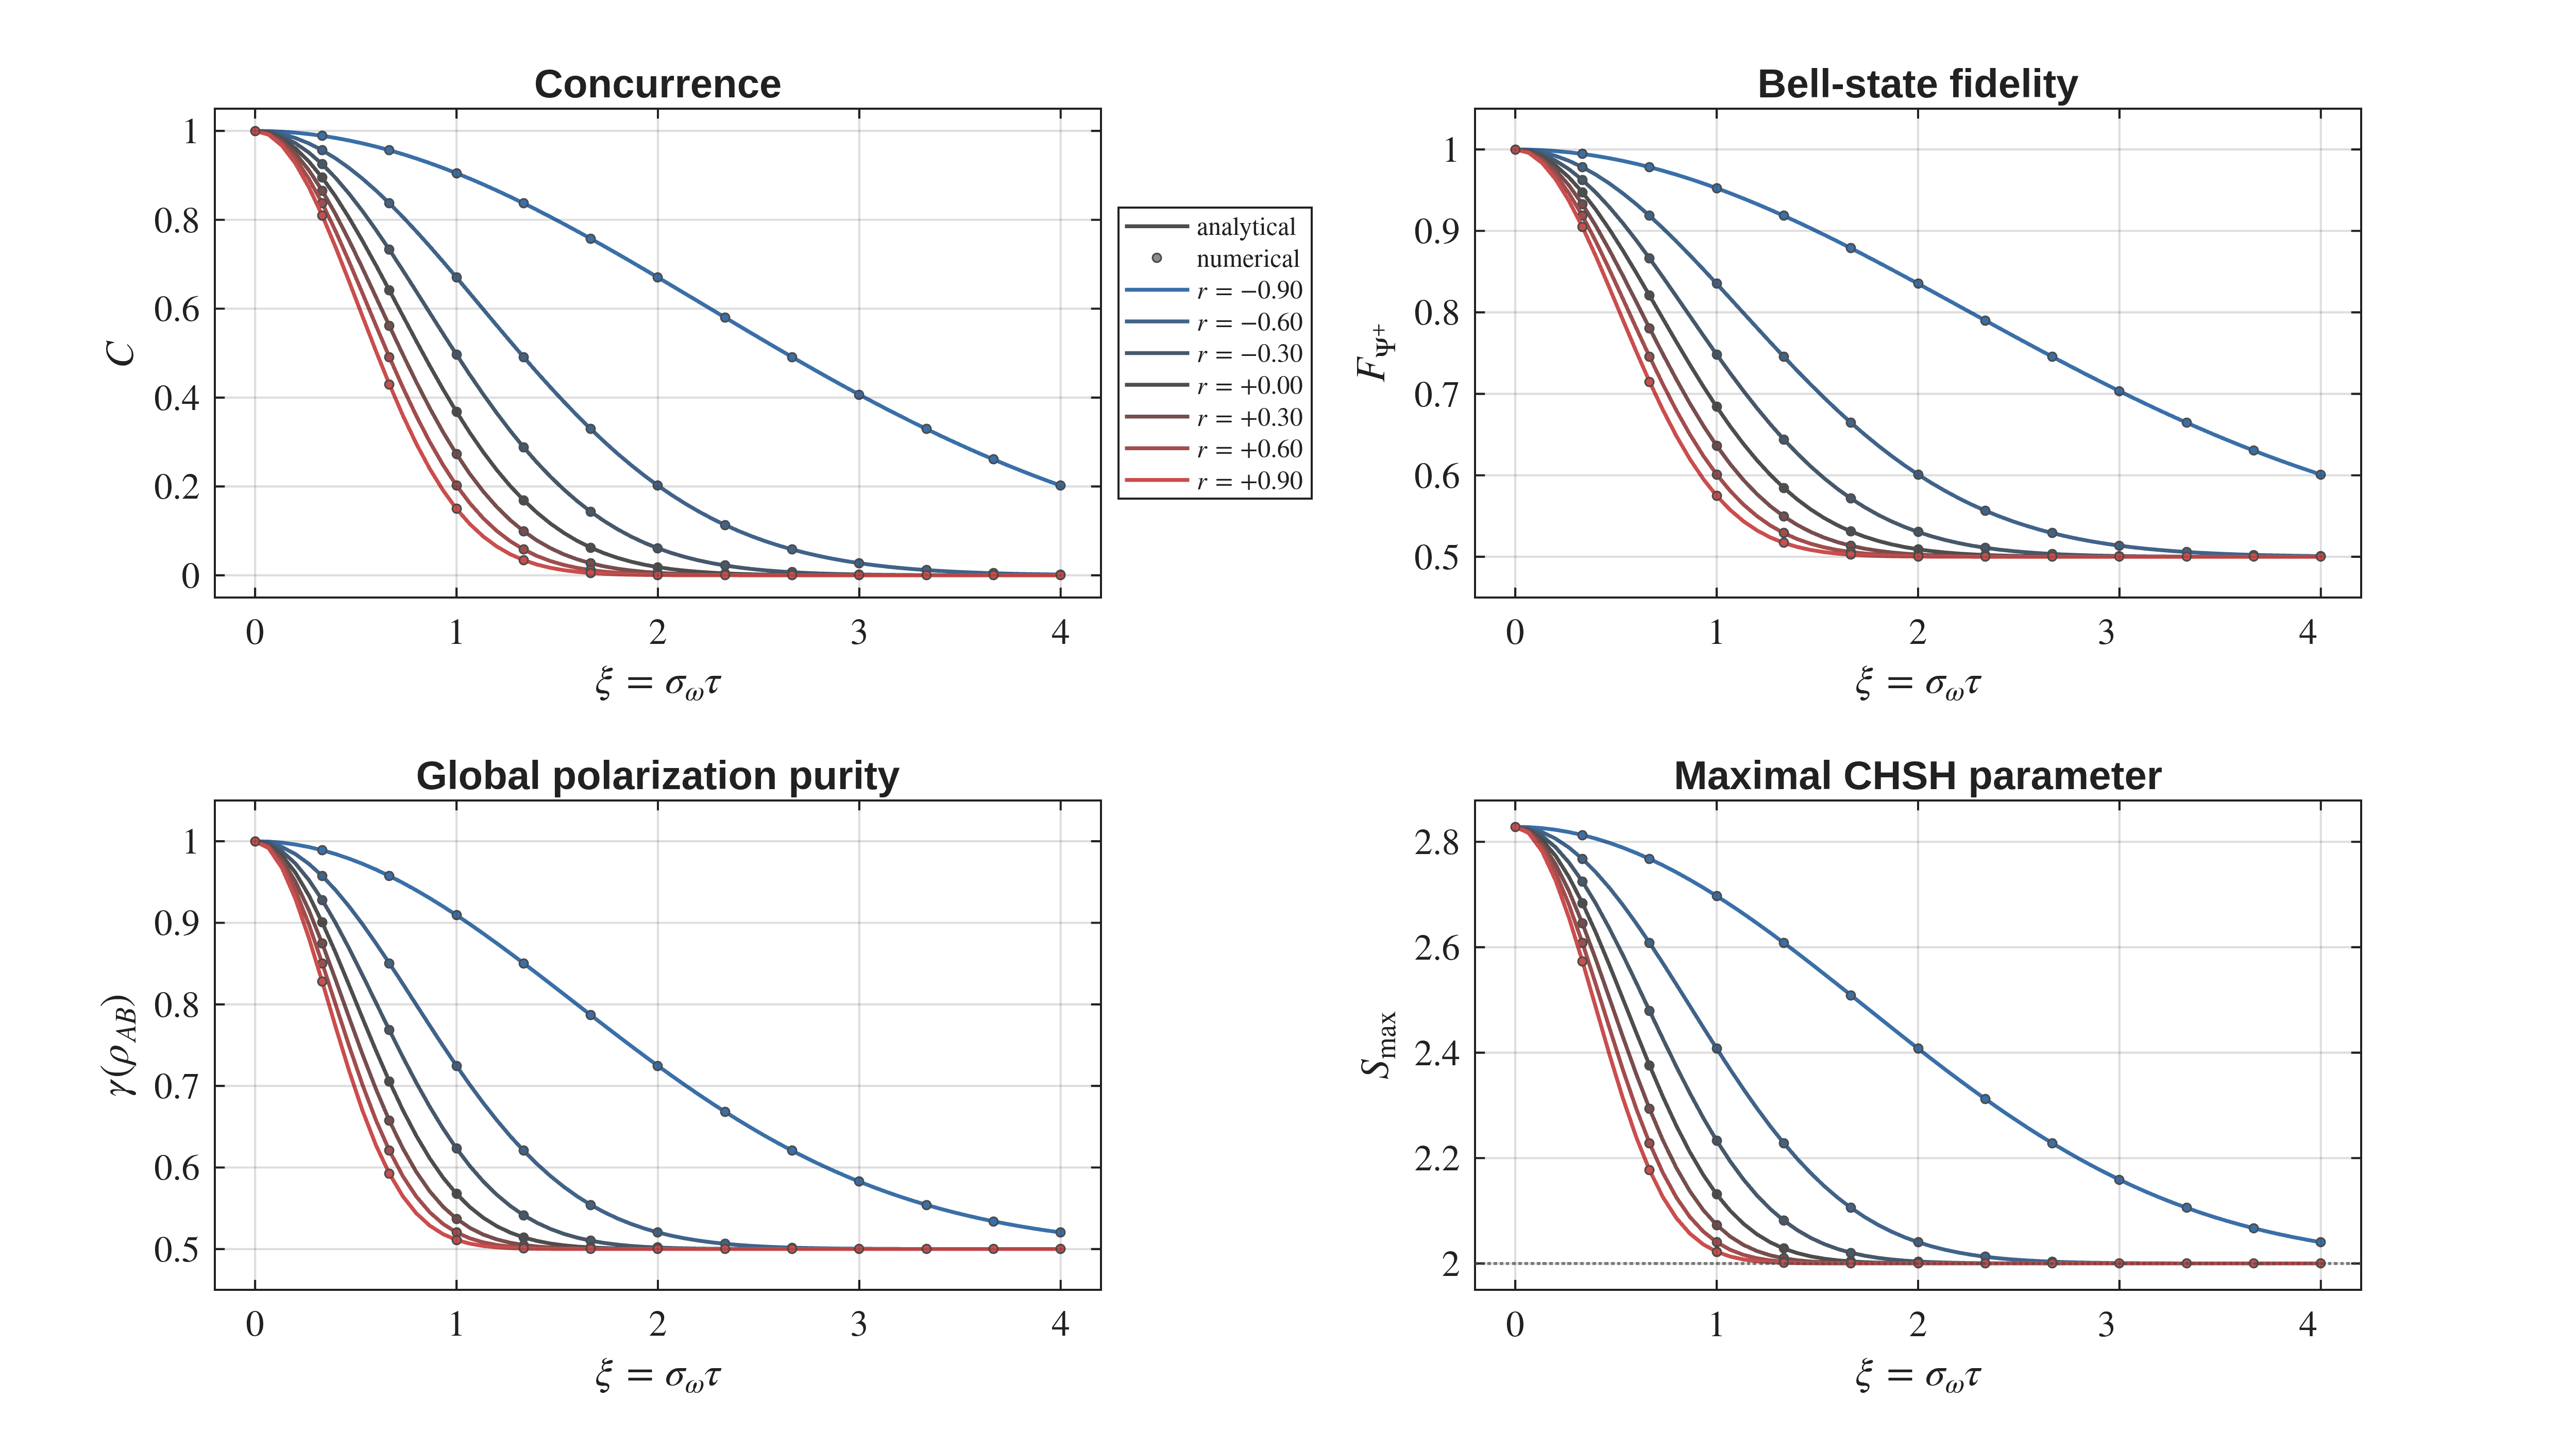
\includegraphics[
        width=\textwidth
    ]{
        figures/experiment_2/experiment_2_two_arm_pmd_spectral_correlations_summary.png
    }

    \caption{
    State metrics for two-arm PMD as a function of the normalized PMD strength
    \(\xi=\sigma_\omega\tau\), for representative spectral-correlation coefficients
    \(r\). Analytical predictions are shown as continuous curves and numerical
    spectral-trace results as markers. Frequency anticorrelation significantly slows
    the degradation of polarization entanglement, whereas positive spectral
    correlation accelerates it.
    }
    \label{fig:exp2_two_arm_pmd_summary}
\end{figure}

For \(r=0\), Eq.~\eqref{eq:exp2_coherence_normalized} reduces to

\begin{equation}
g(\xi,0)=e^{-\xi^2}.
\end{equation}

Compared with the single-arm result \(e^{-\xi^2/2}\), the coherence therefore
decreases more rapidly because both independent PMD contributions enter the
relative phase variance.

The situation changes substantially when the frequencies are anticorrelated.
For example, at \(r=-0.9\),

\begin{equation}
C(\xi,-0.9)
=
e^{-0.1\xi^2},
\end{equation}

so that even at \(\xi=4\),

\begin{equation}
C(4,-0.9)
=
e^{-1.6}
\simeq
0.202.
\end{equation}

By contrast, for \(r=+0.9\),

\begin{equation}
C(\xi,+0.9)
=
e^{-1.9\xi^2},
\end{equation}

and the entanglement rapidly approaches zero.

The same behavior is inherited by fidelity, purity, and CHSH nonlocality through
Eq.~\eqref{eq:exp2_analytical_metrics}. In particular, as \(g\rightarrow0\),

\begin{equation}
F_{\Psi^+}\rightarrow\frac{1}{2},
\qquad
\gamma(\rho_{AB})\rightarrow\frac{1}{2},
\qquad
S_{\max}\rightarrow2.
\end{equation}

The local states remain maximally mixed throughout the entire experiment,
\(\rho_A=\rho_B=I/2\). The degradation therefore appears exclusively in the
two-photon coherence and correlations rather than through the development of a
preferred local polarization state.

%--------------------------------------------------------
% Spectral-correlation regime map
%--------------------------------------------------------

\subsection{Spectral-Correlation Regimes}

The combined dependence on PMD strength and spectral correlation is shown in
Fig.~\ref{fig:exp2_two_arm_pmd_regime_map}.

\begin{figure}[htbp]
    \centering

    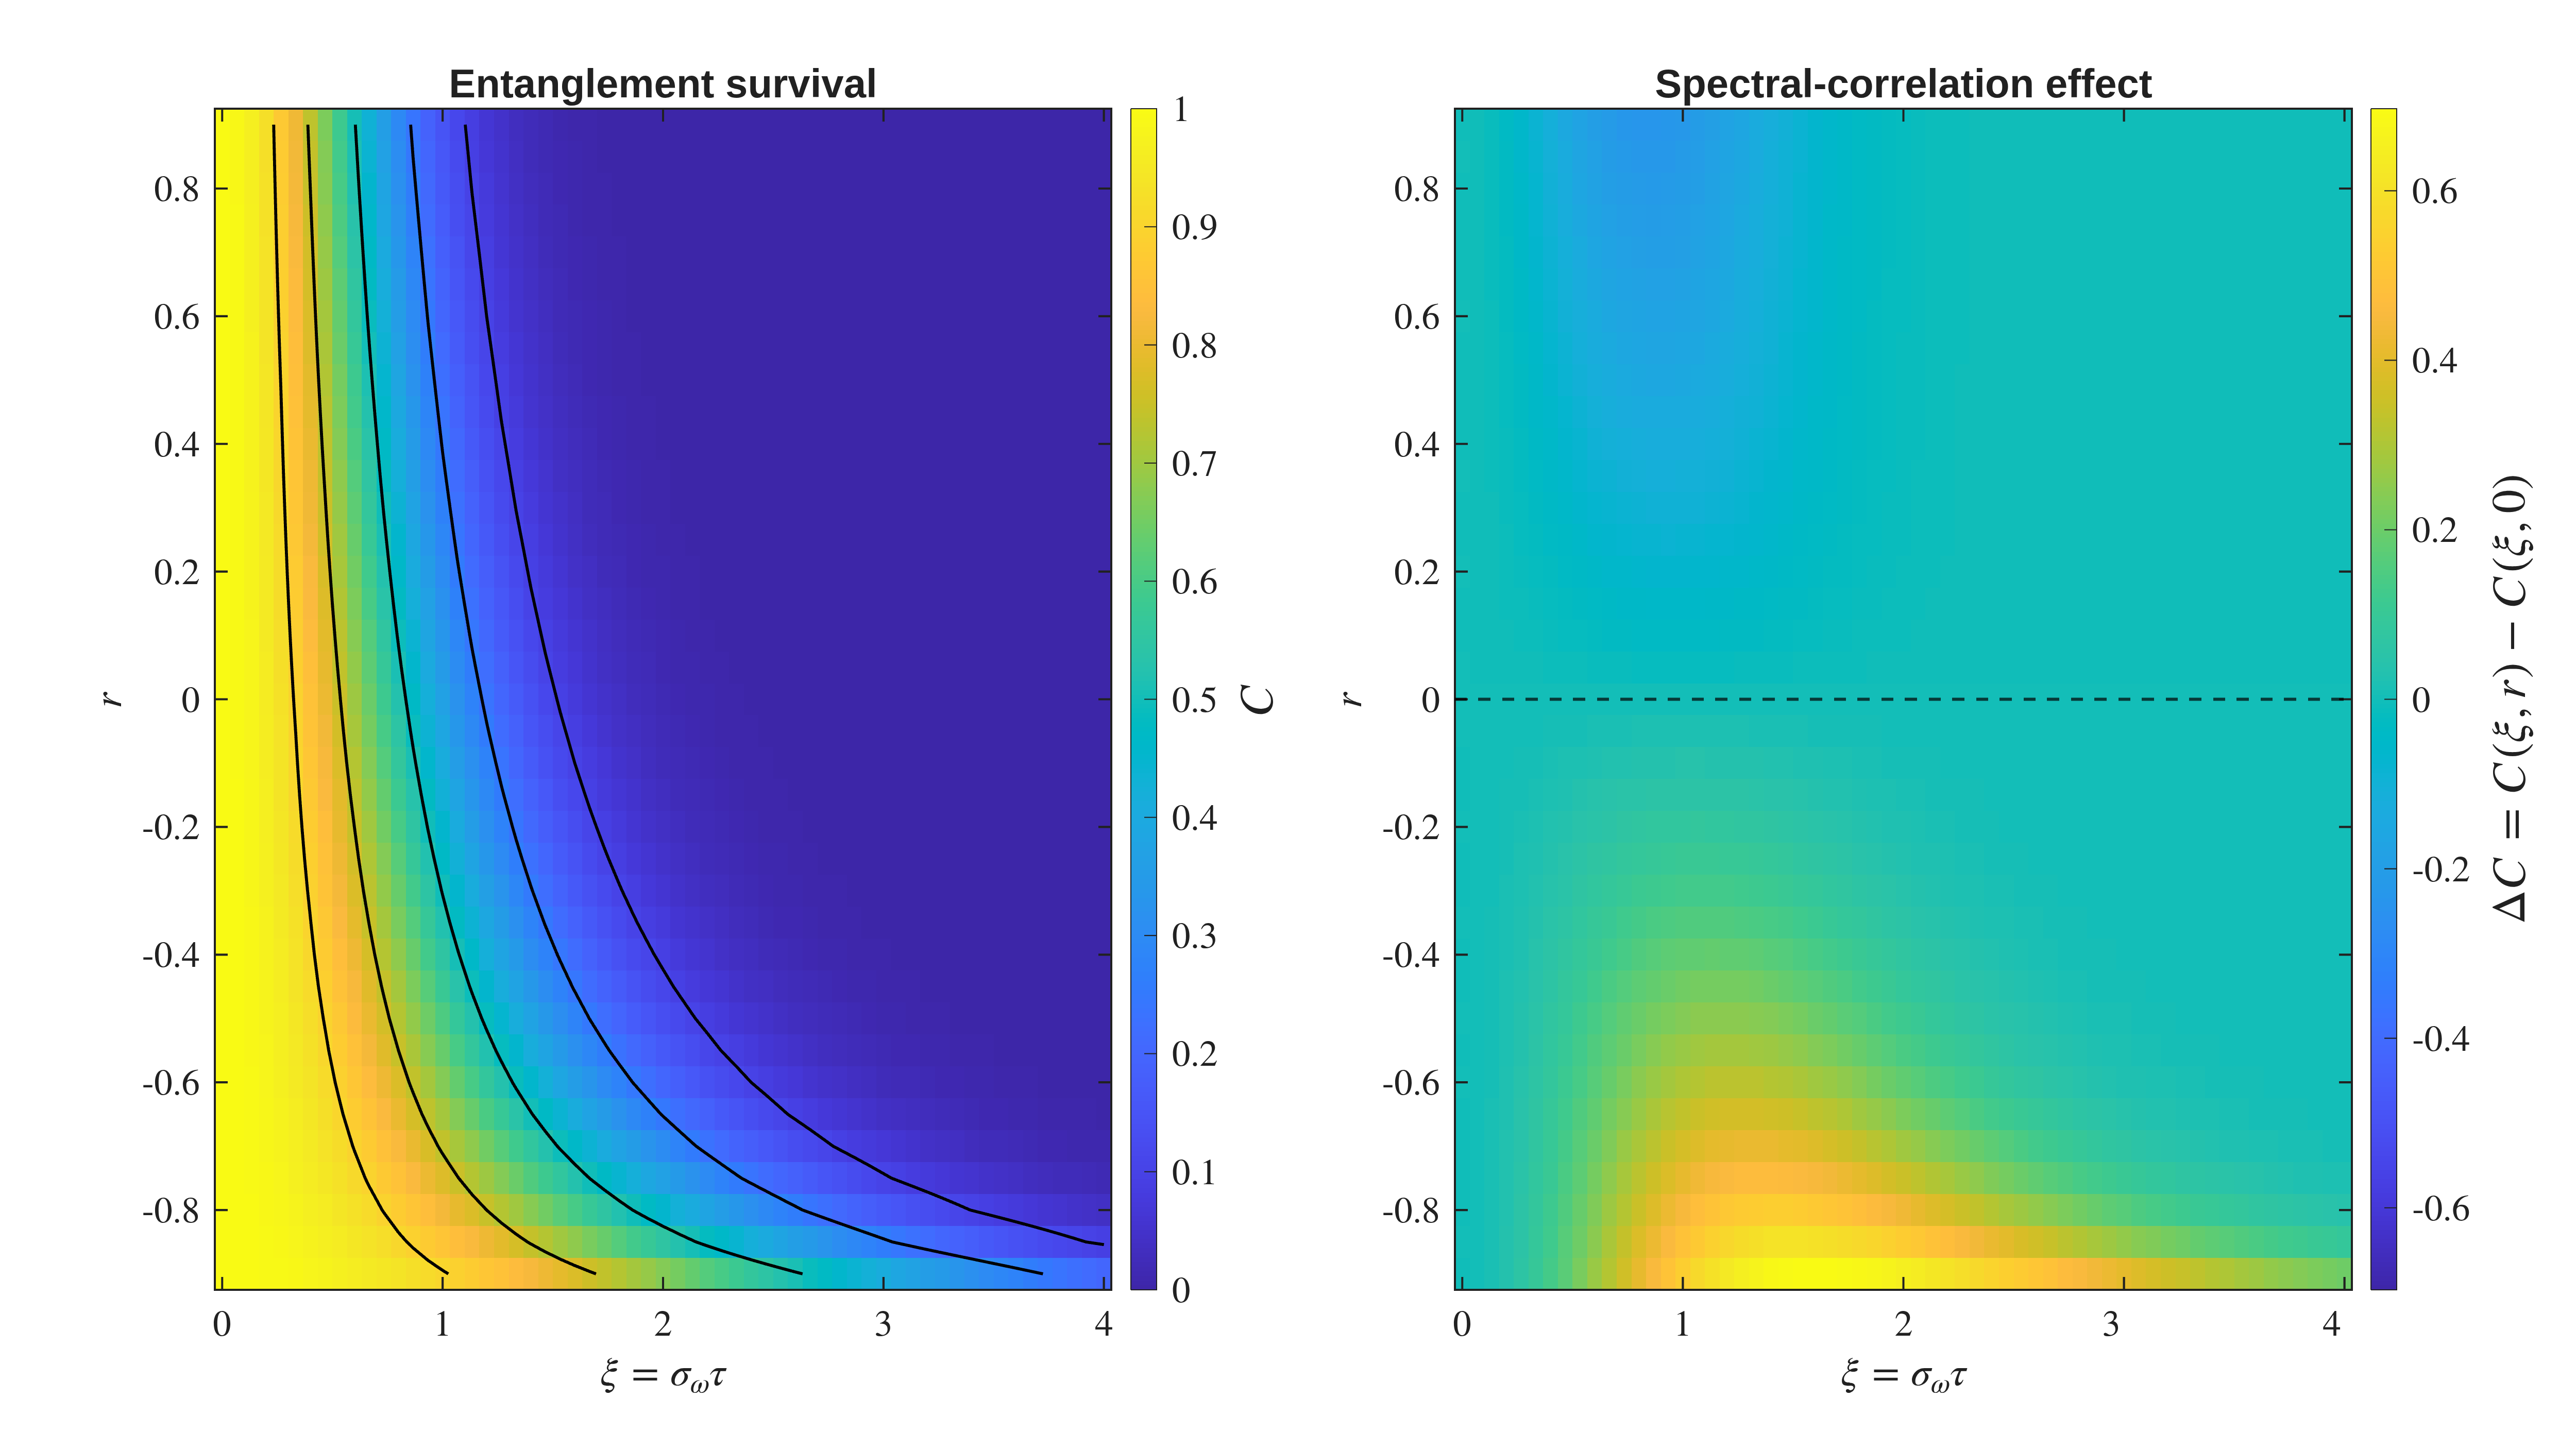
\includegraphics[
        width=\textwidth
    ]{
        figures/experiment_2/experiment_2_two_arm_pmd_spectral_correlations_regime_map.png
    }

    \caption{
    Two-arm PMD spectral-correlation regimes. The left panel shows the
    numerically evaluated concurrence \(C(\xi,r)\), with analytical
    constant-concurrence contours superimposed. The right panel shows the change in
    concurrence relative to an uncorrelated spectrum,
    \(\Delta C=C(\xi,r)-C(\xi,0)\). Negative spectral correlation produces a
    positive entanglement-survival contribution, while positive correlation
    accelerates PMD-induced degradation.
    }
    \label{fig:exp2_two_arm_pmd_regime_map}
\end{figure}

The regime map makes the role of the joint spectrum particularly clear. Since

\begin{equation}
\operatorname{Var}(\Omega_A+\Omega_B)
=
2\sigma_\omega^2(1+r),
\end{equation}

frequency anticorrelation reduces the variance of the spectral combination to which
the polarization state is sensitive. Consequently, the random relative phase is
partially suppressed and a larger fraction of the polarization coherence survives the
spectral trace.

The effect can be isolated by defining

\begin{equation}
\Delta C(\xi,r)
=
C(\xi,r)-C(\xi,0),
\label{eq:exp2_concurrence_gain}
\end{equation}

which analytically gives

\begin{equation}
\Delta C(\xi,r)
=
e^{-(1+r)\xi^2}
-
e^{-\xi^2}.
\label{eq:exp2_concurrence_gain_analytical}
\end{equation}

Therefore,

\begin{equation}
\Delta C
\begin{cases}
>0, & r<0,
\\
=0, & r=0,
\\
<0, & r>0.
\end{cases}
\end{equation}

The improvement for \(r<0\) is not the consequence of a local reduction of the PMD
in either fiber. Each photon still undergoes a frequency-dependent polarization
transformation. Instead, the joint spectral structure correlates the two local
transformations such that their contributions to the relative Bell-state phase
partially cancel.

In the ideal limit \(r\rightarrow-1\),

\begin{equation}
\Omega_A+\Omega_B\rightarrow0,
\end{equation}

and therefore

\begin{equation}
g(\xi,r)\rightarrow1.
\end{equation}

The polarization entanglement can then remain unaffected despite finite PMD in both
arms. This constitutes a nonlocal compensation effect originating from spectral
correlations rather than from an active polarization correction applied after
propagation.

%--------------------------------------------------------
% Numerical validation
%--------------------------------------------------------

\subsection{Numerical Validation}

The numerical spectral trace was compared over the complete
\((\xi,r)\) parameter domain with the continuous Gaussian expressions derived
above. The maximum absolute discrepancies are reported in
Table~\ref{tab:exp2_validation_errors}.

\begin{table}[htbp]
    \centering
    \caption{
    Maximum absolute numerical errors in Experiment~2 relative to the continuous
    Gaussian analytical solution.
    }
    \label{tab:exp2_validation_errors}

    \begin{tabular}{lc}
        \hline
        Quantity & Maximum absolute error
        \\
        \hline

        Global purity
        & \(6.584\times10^{-9}\)
        \\

        Local purity, arm \(A\)
        & \(9.326\times10^{-15}\)
        \\

        Local purity, arm \(B\)
        & \(9.326\times10^{-15}\)
        \\

        Bell-state fidelity
        & \(3.728\times10^{-9}\)
        \\

        Concurrence
        & \(7.456\times10^{-9}\)
        \\

        Tangle
        & \(1.317\times10^{-8}\)
        \\

        Entanglement of formation
        & \(1.031\times10^{-8}\)
        \\

        Maximum CHSH parameter
        & \(9.870\times10^{-9}\)
        \\

        \(c_{xx}\)
        & \(7.456\times10^{-9}\)
        \\

        \(c_{yy}\)
        & \(7.456\times10^{-9}\)
        \\

        \(c_{zz}\)
        & \(9.326\times10^{-15}\)
        \\

        Correlation tensor, Frobenius norm
        & \(1.054\times10^{-8}\)
        \\

        \hline
    \end{tabular}
\end{table}

All discrepancies remain of order \(10^{-8}\) or smaller, while the longitudinal
correlation and local purities agree to approximately machine precision. The
agreement confirms that the finite spectral grid and discrete joint-spectrum
averaging accurately reproduce the continuous Gaussian model over the complete
parameter range considered.

%--------------------------------------------------------
% Physical interpretation
%--------------------------------------------------------

\subsection{Physical Interpretation}

Experiment~2 demonstrates that PMD-induced polarization decoherence cannot in
general be characterized by the marginal bandwidths and individual fiber DGDs
alone. When both photons propagate through frequency-dependent channels, the
joint spectral statistics determine how the two local transformations combine after
the spectral degrees of freedom are discarded.

For the opposite-axis configuration considered here, the relevant spectral variable is
the sum \(\Omega_A+\Omega_B\). Anticorrelated photon pairs exhibit reduced
fluctuations of this quantity and therefore retain a larger polarization coherence.
Positively correlated photons instead increase the corresponding phase variance and
accelerate entanglement degradation.

The experiment thus provides a direct numerical illustration of an important
difference between independent and correlated effective channels. Even though the
fiber transformations remain local,

\begin{equation}
U_A(\Omega_A)\otimes U_B(\Omega_B),
\end{equation}

their effective action on the reduced polarization state is not independent when
\(\Omega_A\) and \(\Omega_B\) are statistically correlated.

Spectral correlations can therefore act as a resource for entanglement distribution:
they do not eliminate PMD locally, but can strongly suppress its observable effect on
the distributed bipartite polarization state.